% DO NOT COMPILE THIS FILE DIRECTLY!
% This is included by the other .tex files.

\begin{frame}[t,plain]
\titlepage
\end{frame}

\begin{frame}
    \frametitle{Objectives of this module}
    \begin{itemize}
        \item How evidences can be useful for defense
        \item Why is contextualisation important
        \item What options do we have in MISP
        \item Best practises to encode and contextualise
        \item How can it be leveraged
    \end{itemize}
\end{frame}

\section{How evidences can be useful for defense}
\begin{frame}
    \frametitle{How evidences can be useful for defense}
    The most common recommendations to protect people and assets from cyber attacks are usually:
    \begin{enumerate}
        \item Maintaining softwares up to date
        \item Staff awareness
        \item Relliable Backups
        \item Endpoints protection tools (IDS or SIEM)
    \end{enumerate}

    \note[item]{An Intrusion Detection System (IDS) is an tools aims at detecting vulnerability exploits or suspicious activity against a server or service}
    \note[item]{A Security Information and Event Management (SIEM) allows to detect and prevent action against cyber attacks}

\end{frame}

\begin{frame}
    \frametitle{How evidences can be useful for defense}
    \begin{itemize}
        \item For an analyst/operator, we can only help endpoints protection tools
        \item With the proper knowledge and methods, it is possible the maximize their accuracy and performance
    \end{itemize}

    These systems can rely on information extracted from
    \begin{itemize}
        \item Log files
        \item Network captures
        \item Disk forensic
        \item ...
    \end{itemize}
    
    However, from a MISP user perspective the hardest part in not to encode the raw evidences, it is to encode them so that they become \textbf{actionable}
\end{frame}

\section{Why is contextualisation important}
\begin{frame}
    \frametitle{Why is contextualisation important}
    \begin{itemize}
        \item Allow the distinction between information of interest and raw data
        \item provide guidance on how to use this information can be used for for protection
        \item Filter out noise from information unralated from your use-case / activity
        \item Enable risk assessment based on attack type, TTP and threat actor
        \item Allow triage in large volume of data
        \item Allow false-positive management
    \end{itemize}

    \note[item]{Tactics, Techniques and Procedures (TTP) describe the context and a detailed description of the behavior taken by an actor}
\end{frame}

\begin{frame}
    \frametitle{What are the expectations of the recipients}
    \begin{itemize}
        \item Being able to consume the data
        \item Find information is relevant for them and their partners
        \item Being able to undetstand the data and its classification
        \item Gauge the credibility, likelyhood and origin of the data
    \end{itemize}

\end{frame}

\begin{frame}
    \frametitle{What do recipient hope to do with the data}
    \begin{itemize}
        \item Being able to filter data efficiently for different use-cases
        \item Obtain as much knowledge out of the data as possible
        \item Know how this data was produce and where it comes from
        \item Deduce why is the data relevant for them and how critical it is
    \end{itemize}
\end{frame}

\begin{frame}
    \frametitle{Is context really that important?}
\begin{lstlisting}
1.2.3.9
137.221.106.104
28c643a1f69f9fca9481a4bc9f3f38f3
4478328408cf3c38b356eed6e86171a5c879663d79867c2b55ec8a0538d7588d
5ef9515e8fd92a254dd2dcdd9c4b50afa8007b8f
81de431987304676134138705fc1c21188ad7f27edf6b77a6551aa693194485e
904afe59f6438848be96fd26fdeab01267070d25
b6c12d88eeb910784d75a5e4df954001
evil.org
accounting.xlsx.exe
cat.jpg.exe
\end{lstlisting}

    \begin{itemize}
        \item Raw data IS useful but useless if you don't know what it is about
        \item That's why the data should carry how and why it's relevant
        \item In MISP, all data intrinsically have some context
        \begin{itemize}
            \item \textbf{Type}: \texttt{ip-src} / \texttt{sha1} / \texttt{domain}
            \item \textbf{Category}: \texttt{network-activity} / \texttt{payload-delivery} / \texttt{external-analysis}
            \item \textbf{to\_ids}: \texttt{yes} / \texttt{no}
        \end{itemize}
    \end{itemize}
    
    \note[item]{The `to\_ids` flag is used to differentiate between indicators and supporting data. If the flag is set, it means the attribute is an indicator and is meant for protective tools.}
\end{frame}

\begin{frame}
    \frametitle{Is context really that important?}
    \begin{itemize}
        \item It should be noted that sometime, more contextual information is not needed as they inherently convey their context:
        \begin{itemize}
            \item Tor exit nodes
            \item Botnet / C2 trackers
            \item Ransomwares' bitcoin addresses
            \item ...
        \end{itemize}
        \item But most of the time, context is essential
    \end{itemize}
\end{frame}
\end{frame}

\begin{frame}
    \frametitle{What sort of context is pertinent}
    \begin{itemize}
        \item To what kind of user this data is for
        \item What type of action can be performed with it 
        \item Data accuracy, reliability and likelyhood
        \item What are the impacts?
        \item For threat actors:
        \begin{itemize}
            \item Who is it? What tools were used?
            \item What are they motivations? Who are their targets?
        \end{itemize}
        \item How can we prevent/detect/block/remediate the attack
    \end{itemize}
\end{frame}

\section{What options do we have in MISP}
\begin{frame}
    \frametitle{What options do we have in MISP}
    MISP offers
    \begin{itemize}
        \item Taxonomies
        \item Galaxies and Galaxy Clusters
        \item MITRE ATT\&CK
        \item MISP Objects and relationships
        \item Sightings and \texttt{first\_seen} / \texttt{last\_seen}
    \end{itemize}
\end{frame}

\begin{frame}
    \frametitle{Taxonomies}
    \begin{itemize}
        \item Simple labels Standardised on vocabularies
        \item Different organisational/community cultures require different nomenclatures
        \item Triple tag system: \texttt{namespace:predicate="value"}
        \item Taxonomy tags often {\bf self-explanatory}
        \begin{itemize}
            \item \texttt{workflow:state="draft"}
            \item doesn\'t need more explanation
        \end{itemize}
        \item JSON libraries that can easily be defined without the involment of the MISP-project team
    \end{itemize}
    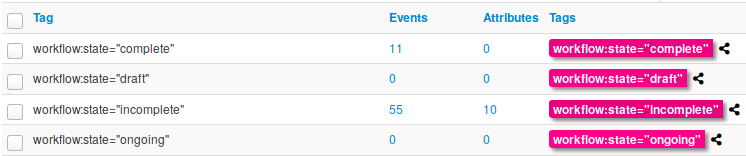
\includegraphics[width=1.0\linewidth]{pictures/taxonomy-workflow.png}
\end{frame}

\begin{frame}
    \frametitle{Galaxies and Galaxy Clusters}
    \begin{itemize}
        \item[\textbf{Galaxy}] Container to group galaxy clusters of the same type
        \item[\textbf{Galaxy Cluster}] knowledge-base item with complex meta-data aimed for human consumption
    \end{itemize}
    \begin{itemize}
        \item Community driven \textbf{knowledge-base libraries used as tags}
        \item Including descriptions, links, synonyms, meta information, etc. 
        \item \textbf{Flexible} and \textbf{reusable}
        \item Works the exact same way as taxonomies but with more meta-data
        \begin{itemize}
            \item \texttt{misp-galaxy:ransomware="CryptoLocker"}
            \item Contains description, reference, documentation and other meta-data
        \end{itemize}
    \end{itemize}
    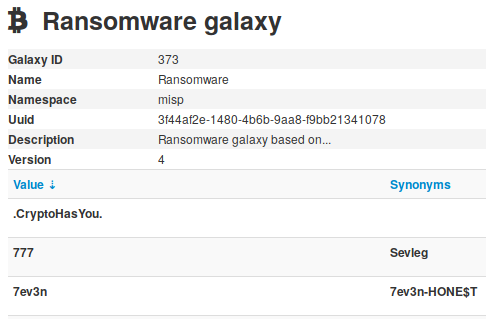
\includegraphics[scale=1.0]{pictures/galaxy-ransomware.png}
\end{frame}

\begin{frame}
    \frametitle{MITRE ATT\&CK and Galaxy Matrices}
    \begin{itemize}
        \item MITRE ATT\&CK is one of the best knowledge base of adversary TTPs
        \item Widely used and supported by a lot of tools
        \item The catalogue includes a matrix-like interface
        \item Offers clear visualisation for the kill chain
    \end{itemize}
    \note[item]{The kill chain are the sequential steps that adversaries can perform in order to achieve an attack}
    \begin{itemize}
        \item MISP Fully support ATT\&CK and embraced it's matrix structure
        \item Multiples matrix for other concerns are available:
        \begin{itemize}
            \item \texttt{Badhra} Similar to ATT&CK but for telecom operators
            \item \texttt{attck4fraud} Regrouped clusters related to fraud actions
        \end{itemize}
    \end{itemize}
    \includegraphics[scale=1.0]{pictures/attacks.png}
\end{frame}

\begin{frame}
    \frametitle{MISP Objects}
    Atomic attributes are great, but are lacking a way to express that some can be related to others.

    MISP Objects are there to fill the gap:
    \begin{itemize}
        \item Template system to build complex structures composed of attributes
        \item Logically group attributes that are contextually linked between each others
        \begin{itemize}
            \item A file object can contain: a size, name, content, cryptographic hashes, etc.
            \item A car object can contain: a brand, a model, a license plate, etc.
        \end{itemize}
    \end{itemize}
    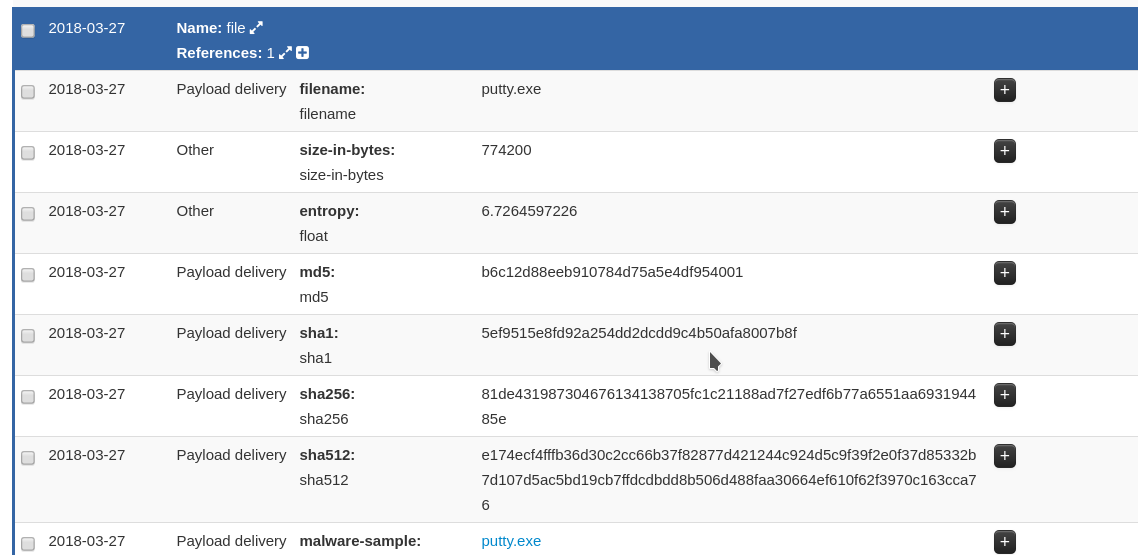
\includegraphics[scale=1.0]{pictures/object.png}
\end{frame}

\begin{frame}
    \frametitle{Relationships}
    \begin{itemize}
        \item Analysts want more than a table of atrtibute, they want to see how each of them interact with the others
        \item Relationships are essentials to describe scenarios or stories with the data
        \item MISP allow these relationship to be built between objects
    \end{itemize}
    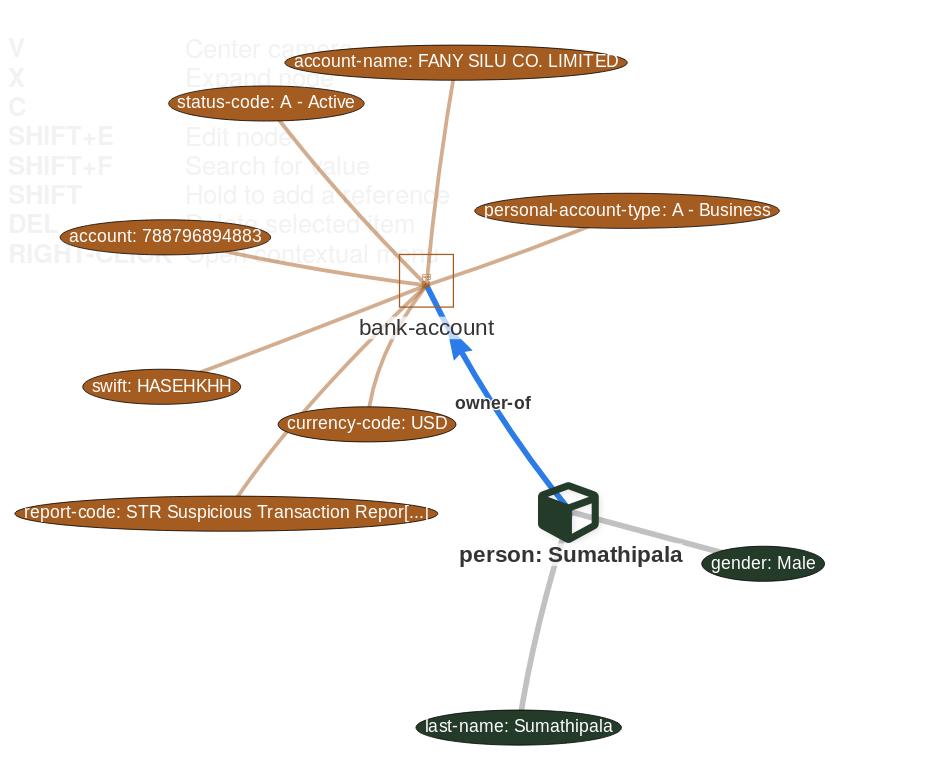
\includegraphics[scale=1.0]{pictures/relationship.png}
\end{frame}

\begin{frame}
    \frametitle{Timeliness with Sightings and \texttt{first\_seen} / \texttt{last\_seen}}
    Another aspect often neglected at first is temporality and MISP offerts to ways to avoid having the data frozen in time
    \begin{itemize}
        \item Sightings
        \begin{itemize}
            \item Allows to signal the fact that an indicator was sighted
            \item They can record the time and where they were the sighting was seen
            \item E.g.: Sight C2 servers or phishing websites
        \end{itemize}
        \item \texttt{first\_seen} / \texttt{last\_seen}
        \begin{itemize}
            \item These two data-points allow to set when the specified item was first and last seen
            \item Enables the visualisation of data timeframe with a timeline
            \item E.g.: Track the duration of a campaign or duration for which something was online
        \end{itemize}
        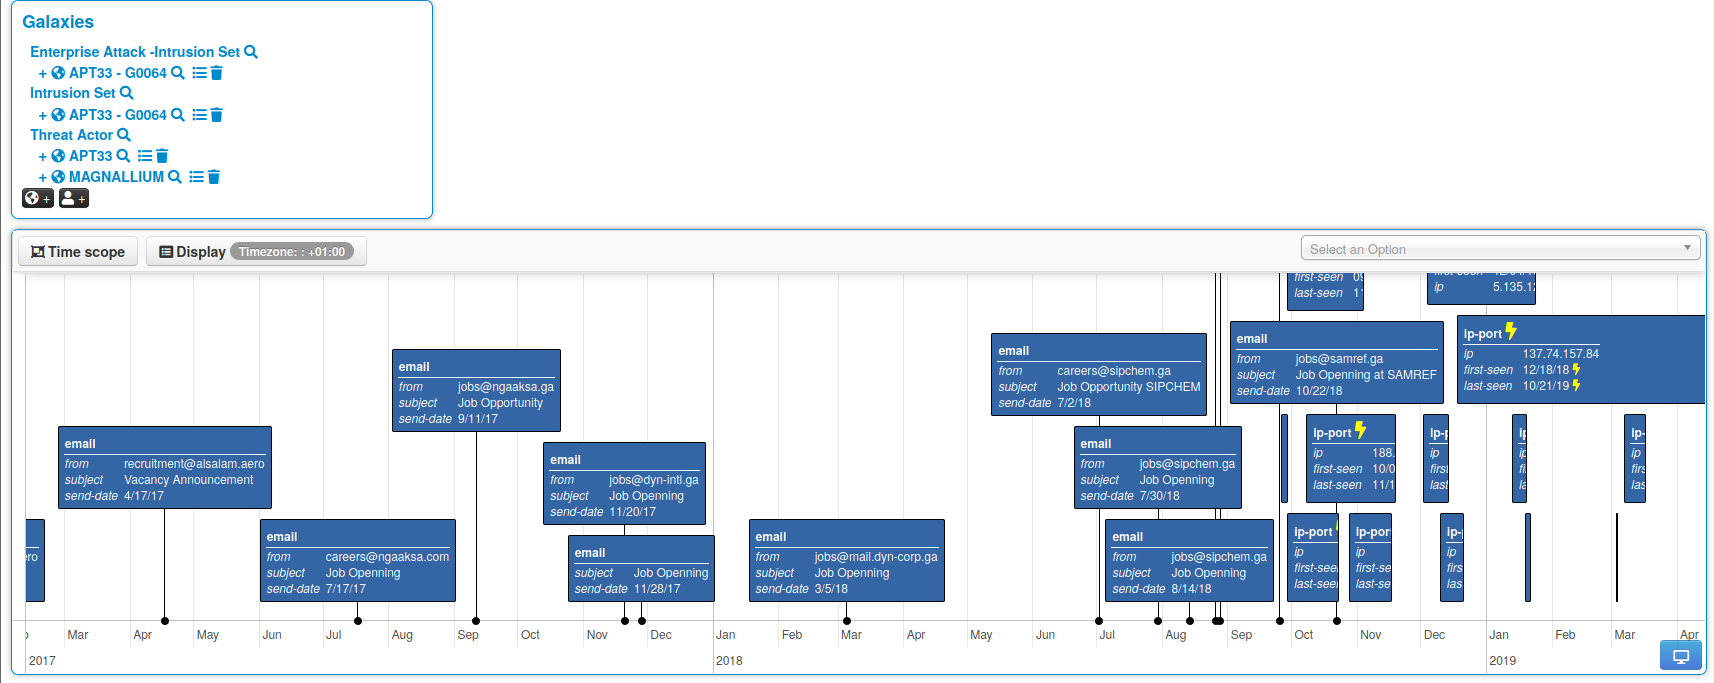
\includegraphics[scale=1.0]{pictures/timeline.png}
    \end{itemize}
\end{frame}

\section{Best practises to encode and contextualise}
\begin{frame}
    \frametitle{Encoding: Event}
    Always keep in mind that the recipient is a human:
    \begin{itemize}
        \item Include a self-explanatory title
        \item Make it concise
        \item Include a report (using event-report) along with the machine parsable data
    \end{itemize}
    That will make the live of the analyst easier: That analyst might end up being you!
\end{frame}

\begin{frame}
    \frametitle{Encoding: Attributes and objects}
    Atomic data by themselve rarely exists: They are often linked to another entity
    \begin{itemize}
        \item Interactions between between elements are frequent
        \begin{itemize}
            \item They can often be described by using verbs: \texttt{connects-to}, \texttt{contain-within}, ...
        \end{itemize}
        \item A story can be inferred without the need to put it into words
        \begin{itemize}
            \item \texttt{file} was attached to \texttt{email} which when extracted contained a \texttt{malware} connecting to \texttt{ip-address} which was used \texttt{C2}
        \end{itemize}
        \item Properly encoding these relationships turns flat data into a connected graph
    \end{itemize}
\end{frame}


\begin{frame}
    \frametitle{Contextualise: Distributions and permissible actions}
    Adding context on what actions can be done on the data and who can it be shared with
    \begin{itemize}
        \item Permissible actions taxonomies:
        \begin{itemize}
            \item \texttt{PAP}: Permissible Actions Protocol
            \item \texttt{IEPF}: Information Exchange Policy (IEP) Framework
        \end{itemize}
        \item Sharing level taxonomies:
        \begin{itemize}
            \item \texttt{TLP}: Traffic Light Protocol
            \item \texttt{IEPF}: Information Exchange Policy (IEP) Framework
        \end{itemize}
    \end{itemize}
\end{frame}

\begin{frame}
    \frametitle{Contextualise: Attributes and their context}
    Each data point has a meaning and tells a part of the story:
    \begin{itemize}
        \item In what context was this IoC seen?
        \item Is it related to compromision? Does it tell us anything about the adversary infrastructure
        \item Was it used to exfiltrate data? Did it acted as a C2?
        \item Did it perform subsequent actions?
        \item ATT&CK can procure even more knowledge
    \end{itemize}

    However, think twice before tagging:
    \begin{itemize}
        \item If a tag applies to the whole content of the event, it should be attached on the event instead
        \item If the tag offers no real utility or hinder your ability to analyse the whole dataset, it should probably be ignored
    \end{itemize}
\end{frame}

